\documentclass[dcc,uchile]{fcfmcourse}
\usepackage{teoria}
\usepackage[utf8x]{inputenc}
\usepackage{amsmath}
\usepackage{amsfonts,setspace}
\usepackage{listings}
\usepackage{hyperref}
\usepackage{color}





\definecolor{pblue}{rgb}{0.13,0.13,1}
\definecolor{pgreen}{rgb}{0,0.5,0}
\definecolor{porange}{rgb}{0.9,0.5,0}
\definecolor{pgrey}{rgb}{0.46,0.45,0.48}

\lstset{language=Java,
  showspaces=false,
  showtabs=false,
  breaklines=true,
  showstringspaces=false,
  breakatwhitespace=true,
  commentstyle=\color{porange},
  keywordstyle=\color{pblue},
  stringstyle=\color{pgreen},
  basicstyle=\ttfamily,
  moredelim=[il][\textcolor{pgrey}]{$ $},
  moredelim=[is][\textcolor{pgrey}]{\%\%}{\%\%}
}
\newcommand{\ptitle}[1]{\underline{\textbf{#1}}}

\newenvironment{codebox} {\small \ttfamily \obeylines \begingroup \setstretch{-2.4}} {\endgroup}

% COmpletar titulo
\title{Auxiliar 12 - Grafos}
\course[CC3001]{Algoritmos y Estructuras de Datos}
\professor{Nelson Baloian}
\professor{Patricio Poblete}
\assistant{Gabriel Azócar, Manuel Cáceres}
\assistant{Michel Llorens, Sergio Peñafiel}


\begin{document}
\maketitle

\vspace{-1ex}


\begin{problems}


\problem \ptitle{Metro de Santiago}
Contabilizando que el plano de un sistema de metro, en específico el del Metro de Santiago, es posible representarlo como un grafo.
\begin{center}
    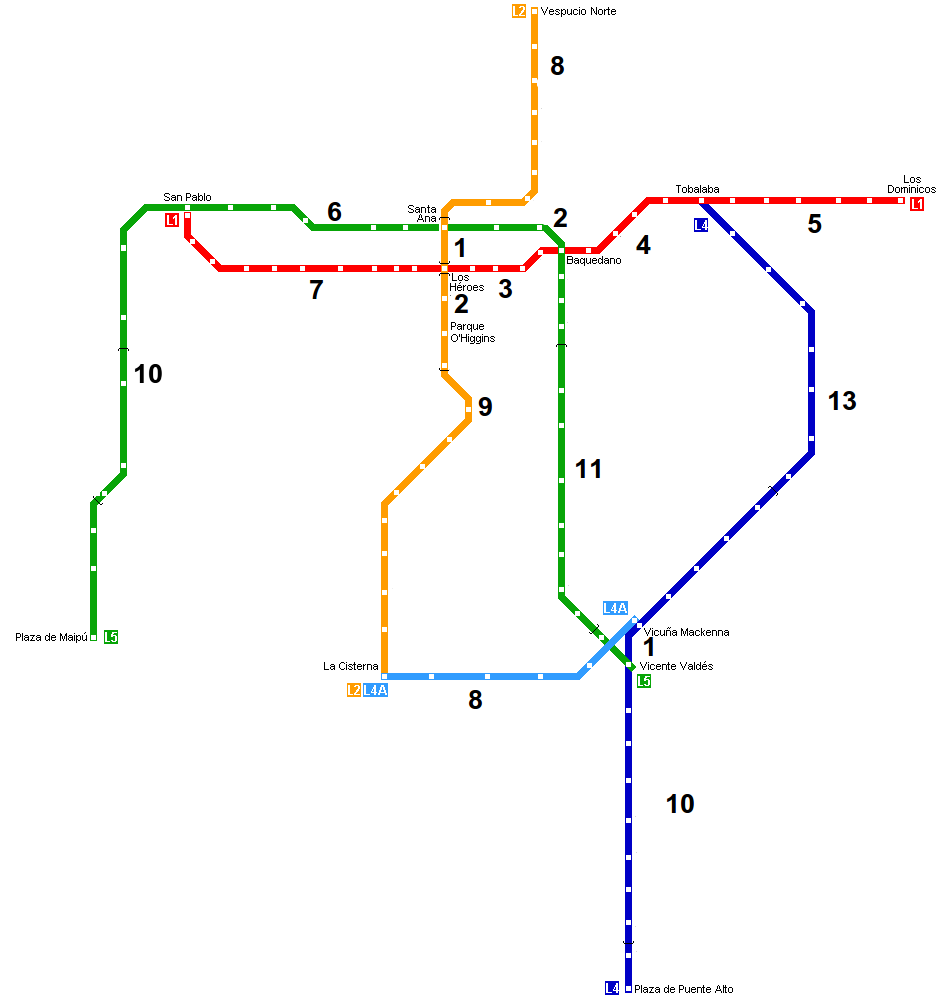
\includegraphics[scale=0.25]{imagenes/metro.png}
\end{center} 
\begin{enumerate}[1)]
    \item ¿Cómo llevaría un plano a un grafo?
    \item ¿Qué importancia tienen las estaciones de combinación? ¿Cómo las representaría?
    \item Calcule el árbol cobertor usando Prim y tomando como nodo inicial Parque O'Higgins.
    \item Calcule el camino más corto desde Plaza de Puente Alto a Parque O'Higgins y a Plaza de Maipú. ¿Es relevante la representación de las estaciones de combinación con esto?
    %Pensar en Vicente Valdés. Cada estación combinación se representa como dos nodos entre los cuales la distancia es 0. La gracia es que a veces las estaciones cierran sólo en una línea y esto no afecta la otra. Por ejemplo a veces la L5 se corta la mitad hasta Vicente inclusive, pero la estación Vicente sigue funcionando para la L4. En la representación tradicional la L4 quedaría cortada al medio.
    \item ¿Es realmente el camino más corto el más rápido? ¿Qué variables pueden afectar esta decisión? 
    % En la pregunta anterior es importante hablar de Waze y cómo contabiliza además los tacos, los accidentes, etc. Lo que hace es primero aplicar Dijkstra en el servidor para el camino más corto (las distancias se ponderan por la velocidad promedio de cada vía), y luego va contabilizando sucesos y los va recalculando en el dispositivo acorde a decisiones del usuario (como no tomar la vía recomendada) e intentando reconectarlo al camino principal, algo así como el camino más corto al camino principal (pensar en Prim).
\end{enumerate}

\newpage
\problem \ptitle{Internet}

Las redes de internet pueden ser vistas como un conjunto de routers que se conectan entre sí y llegan a terminales que pueden ser dispositivos como computadores, servidores, etc. Esta red se puede modelar usando un grafo en el cual cada nodo es un router o terminal y cada arco representa un enlace entre 2 routers o terminales, este enlace además tiene anotado el tiempo que se demora en transmitir 1 Mb de información en milisegundos. Considere que este grafo está almacenado como una matriz de adyacencia en una variable global \texttt{G}, tal que para cualquier celda es 0 si no hay enlace entre los 2 nodos, o $T > 0$ si existe un enlace entre los nodos con tiempo de transmisión $T$.

\begin{enumerate}
    \item k amigos quieren jugar el último juego online del momento, en este juego uno de ellos debe ser el \textit{host} y por lo tanto todos se comunican con él para jugar. Cree la función \texttt{int host(int[] amigos)} que dado los índices que representan los nodos de los terminales de los amigos, entrega el índice del amigo tal que la suma de los tiempos de transmisión a todo los otros amigos es mínima. 
    \item Suponga ahora que todos enlaces pertenecen a alguno de los 3 proovedores de internet que existen, y que estos le dan mayor prioridad a sus clientes, de tal forma que si un usuario que no es cliente del proovedor quiere usar el enlace el tiempo de transmisión se duplica. La información de los dueños de los enlaces está en otra matriz \texttt{P} con la misma forma que \texttt{G} pero que indica 1, 2 o 3 según el proovedor del enlace. Diseñe un algoritmo que le permita a 2 amigos saber cuál es el proovedor de internet que deberían contratar para minimizar su tiempo de transmisión. Para esto cree la función \texttt{int proovedor(int i, int j)} que dado los indices de los nodos de los amigos retorna el indice del proovedor que deberían contratar.
\end{enumerate}

\end{problems}
\end{document}